\documentclass[10pt,twocolumn]{article}
\usepackage{geometry}
\geometry{verbose,headsep=3cm,tmargin=2.5cm,bmargin=2.5cm,lmargin=2.0cm,rmargin=2.0cm}
\usepackage{graphicx}
\usepackage{xcolor}
\usepackage[font=small]{caption}
\usepackage{cleveref}
\usepackage{amsmath,amssymb,latexsym}
\usepackage{marvosym}
\usepackage{url}
\usepackage{lipsum}
\usepackage{bm}
\usepackage{float}
\usepackage[english]{babel}
\usepackage{hyperref}
\usepackage{epsf}
\usepackage{float}
\usepackage{mathpazo}
\usepackage{pifont}
\usepackage{wrapfig}
\usepackage{multicol}
\usepackage{enumitem}
\usepackage{xcolor}
\usepackage{framed}
\usepackage[utf8]{inputenc}
\graphicspath{{DWGs/}}
\usepackage{framed}

% Document font:
\usepackage{charter}

\newcommand{\highlight}[1]{%
  \colorbox{orange!50}{$\displaystyle#1$}}

\begin{document}

%%% HEADER --------------------------------------------------------------
% ------------------------------------------------------------------------

\twocolumn[{
\begin{@twocolumnfalse}

  \begin{center}
%\textcolor{lgray}
    \vskip-5em

    \hfill
    \fontsize{10}{10}\selectfont {\textit{Bruxelles, November 2018}}

    \vskip2ex
    
	\vspace{5ex}
	
    \fontsize{24}{10}\selectfont {Notes on Principal Component Analysis}
   
    
      \vspace{1ex}
   \fontsize{10}{10}\selectfont {camillejr.github.io/science-docs}
          
  \noindent%
    
\vskip1ex

{\rule{\textwidth}{0.5pt}}

  \end{center}
  
\vspace{8mm}

\end{@twocolumnfalse}
}]

%%% HEADER END -----------------------------------------------------------
% ------------------------------------------------------------------------

\vspace{10mm}

\setlength{\parindent}{0cm}

\section*{Preface}

These are notes on \textbf{Principal Component Analysis} (PCA), a technique for finding low-dimensional manifolds in high-dimensional data sets.

This document is still in preparation. Please feel free to contact me with any suggestions, corrections or comments.

\tableofcontents

\section{Motivation for data reduction}

There are several questions which stimulated the development of data reduction techniques and reduced-order modelling:

\begin{enumerate}
\item Can we send less information but preserve the resolution of the data (data compression)?

\item If the data were measurements from an experiment, can we predict what the outcome of another measurement will be?

\item Can we build a model that will make predictions about a system?

\item Can we make sense of a large data set with high-dimensionality (which cannot be plotted graphically)?
\end{enumerate}

\section{Datasets for PCA}

For the rest of this document, we assume that the dataset for performing PCA is structured as follows: each column represends one variable and the rows correspond to variable observations (e.g. at different positions in space, or in time).

\begin{figure}[H]
\centering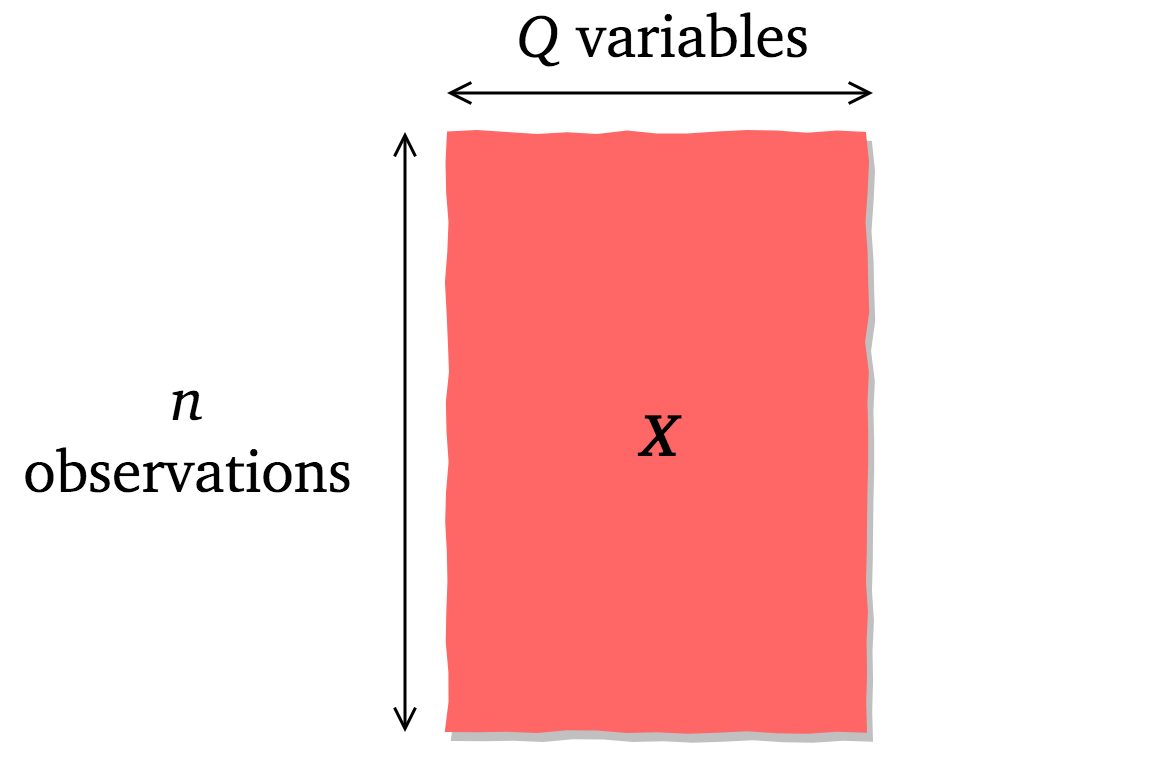
\includegraphics[width=5cm]{data-set-PCA.png}
\caption{Data matrix for PCA.}
\label{fig:data-matrix}
\end{figure}

This is also the data format that is needed for the MATLAB command \texttt{pca}. From the MATLAB documentation:


\begin{framed}
\texttt{pca(X)}

\,\,

Rows of X correspond to observations and columns correspond to variables.
\end{framed}

\section{Covariance matrix}

We start our discussion of PCA with explaining the concept of a \textit{covariance matrix}, since computing this matrix is a starting point for performing PCA.

\begin{figure}[H]
\centering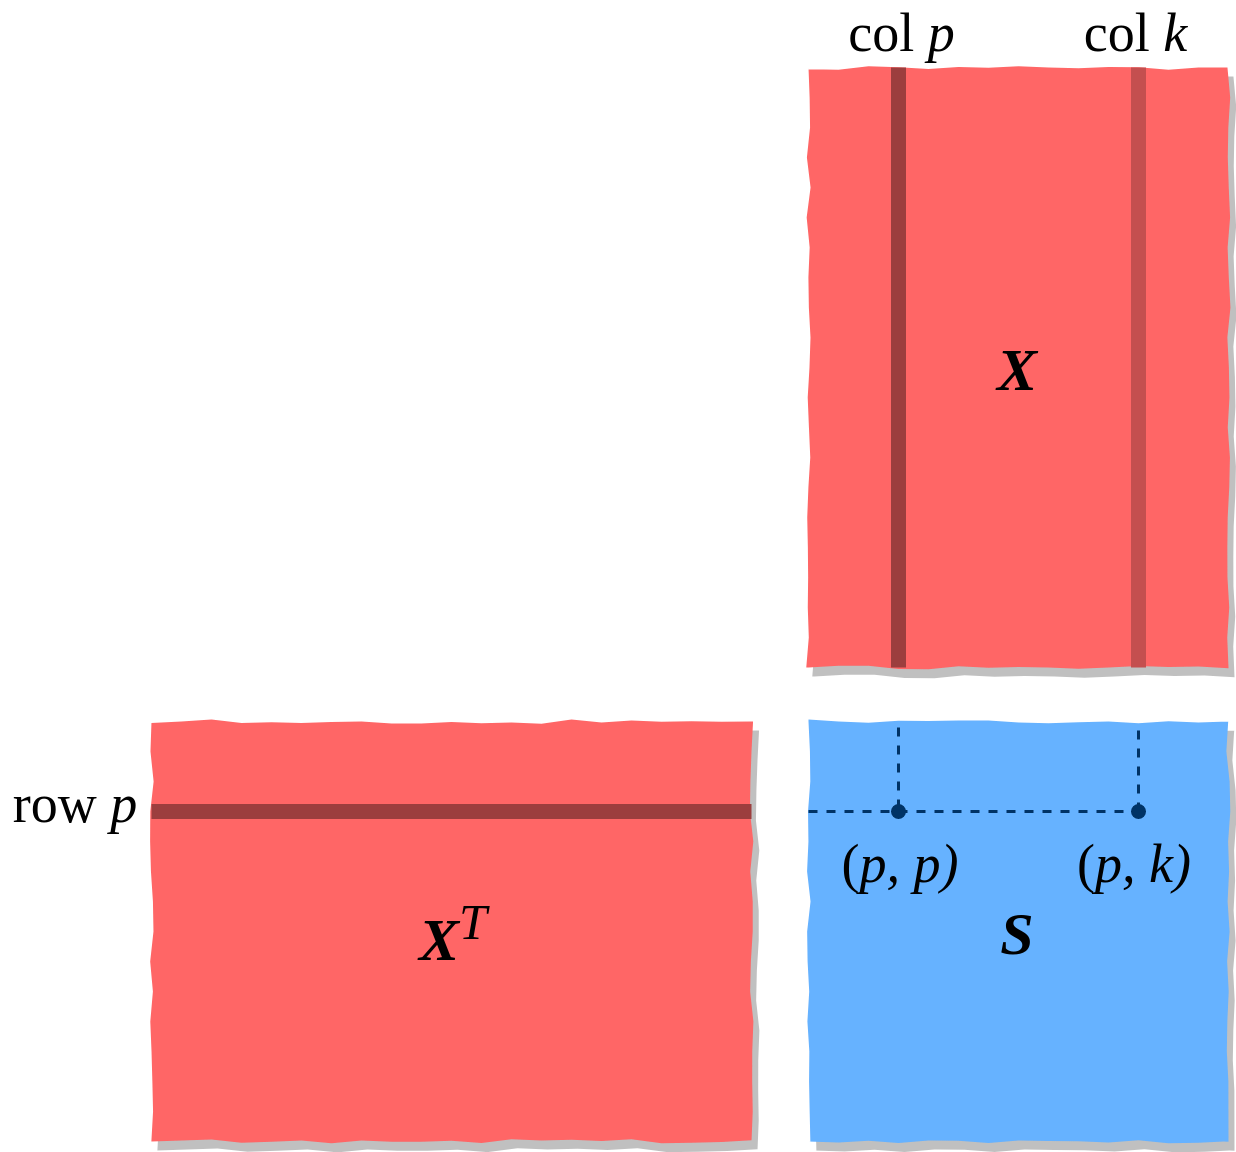
\includegraphics[width=7cm]{cov-matrix.png}
\caption{Covariance matrix $\bm{S}$ graphical interpretation.}
\label{fig:covariance-matrix}
\end{figure}


\begin{equation}
\bm{S} = \frac{1}{n-1} \bm{X^T} \bm{X}
\end{equation}


\section{PCA workflow}





\section{PCA example}

\section{Linear vs. non-linear PCA}

The linear-PCA is adequate for data sets that can be approximated by a linear combination:

\begin{equation}
\text{Data} \approx A_1 \vec{PC1} + A_2 \vec{PC2} + \dots + A_n \vec{PCn}
\end{equation}

where $\vec{PC1}, \vec{PC2}, \dots, \vec{PCn}$ are consecutive principal components (PCs).

The example of a data set that is suited for linear-PCA is presented in Figure \ref{fig:linear_PCA_data}. What is unique about such data set is that it has got a preferred direction in a lower dimension (in this case 1D) along which the data points are aligned. The first PC will be associated with this direction. There will also be a second PC which is perpendicular to the first one, however the weight of this second PC is much lower - there is much less variance of data along this other direction.

The data reduction that we can perform in our heads is that this data set almost aligns with a linear function $f(x) = x$ for $x \in \langle 1; 3 \rangle$.

\begin{figure}[H]
\centering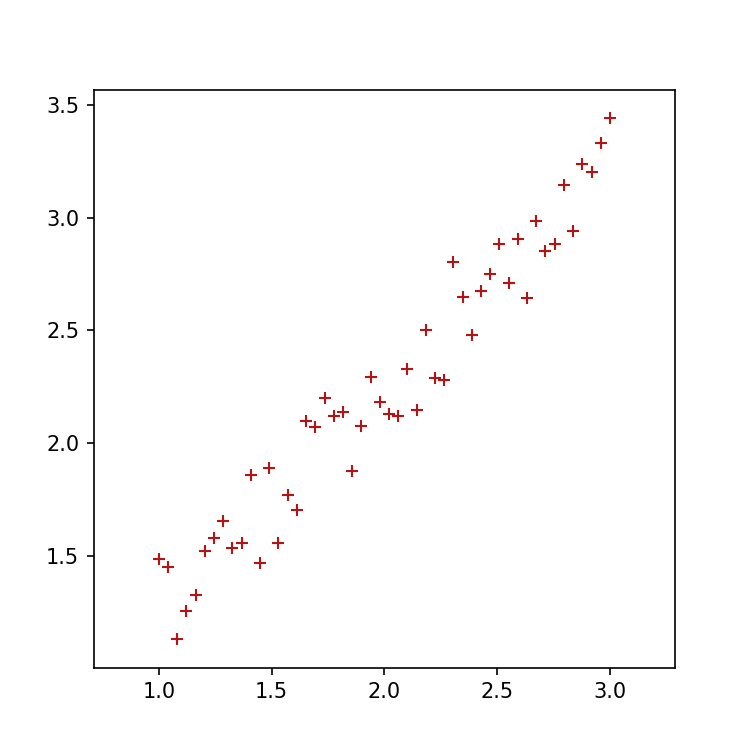
\includegraphics[width=7cm]{../python/PCA-fake-datasets/PCA_linear_scatter_1.png}
\caption{Data set for linear-PCA.}			
\label{fig:linear_PCA_data}
\end{figure}

We may approximate the above data set simply by:

\begin{equation}
\text{Data} \approx A_1 \vec{PC1}
\end{equation}

When we take a look at a data set in Figure \ref{fig:nonlinear_PCA_data}, we can see that the data is spread almost equally along two dimensions. The two PCs of such data set will have almost the same weight (the length of the two eigenvectors will be almost the same). It seems that there is no preferred direction in this data. So, does that mean that it cannot be reduced?

The underlying pattern in this data set is very clearly visible. Intuitively, we can say that the data points are almost aligned with a circle centered at $(2;2)$ with radius $r=1$. If we knew a function $f(x)$ describing that circle, perhaps we might be able to write it in terms of just the first PC and approximate:

\begin{equation}
\text{Data} \approx f(\vec{PC1})
\end{equation}

where $f(\vec{PC1})$ is essentially non-linear.

One idea to find the function $f$ might be to associate the first PC with the radius of the circle (that is find the relation $r(PC1)$) and write:

\begin{equation}
f(x, \vec{PC1})^2 = x^2 + r(\vec{PC1})^2
\end{equation}

This will give us a centered approximation to the original data. 

\begin{figure}[H]
\centering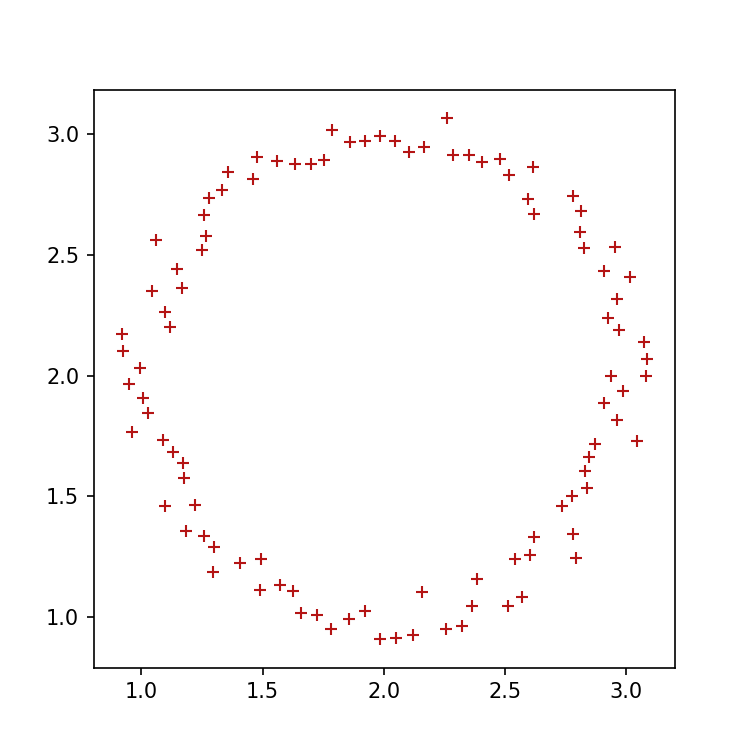
\includegraphics[width=7cm]{../python/PCA-fake-datasets/PCA_nonlinear_scatter_2.png}
\caption{Data set for non-linear-PCA.}			
\label{fig:nonlinear_PCA_data}
\end{figure}

To conclude, the non-linear-PCA is helpful at times when there is no preferred direction in a data set, however there is an underlying non-linear relation that describes the data. The linear-PCA would in such case not give a satisfactory approximation after truncating the number of PCs. 




\appendix

\section{APP1} \label{app:A}

\section{APP2} \label{app:B}

\thebibliography{}

\bibitem{Jolliffe} Ian T. Jolliffe \textit{Principal Component Analysis}, Second Edition, 1986
\bibitem{Strang} Gilbert Strang \textit{Introduction to Linear Algebra}, Fifth Edition, 2016
\bibitem{Shlens} Jonathon Shlens, \textit{A Tutorial on Principal Component Analysis}, 2016, \texttt{https://arxiv.org/abs/1404.1100}

 \label{bib:pope}


\end{document}
